\begin{figure}[t]
\small
    \centering
    \begin{minipage}[c]{.48\textwidth}
    \centering
    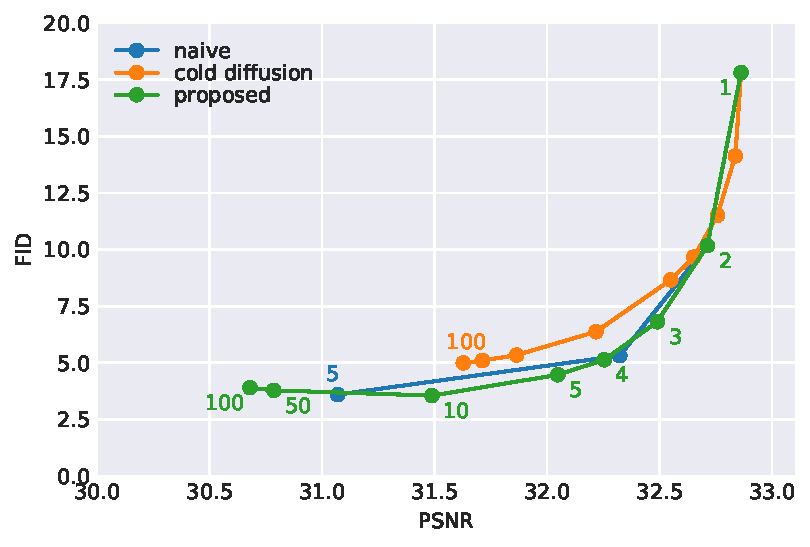
\includegraphics[width=0.95\linewidth]{assets/pd_curve_gopro_sampler.pdf} \vspace{-.5em}
    
    (a) Motion Deblurring (GoPro dataset)
    \end{minipage}
    \begin{minipage}[c]{.48\textwidth}
    \centering
    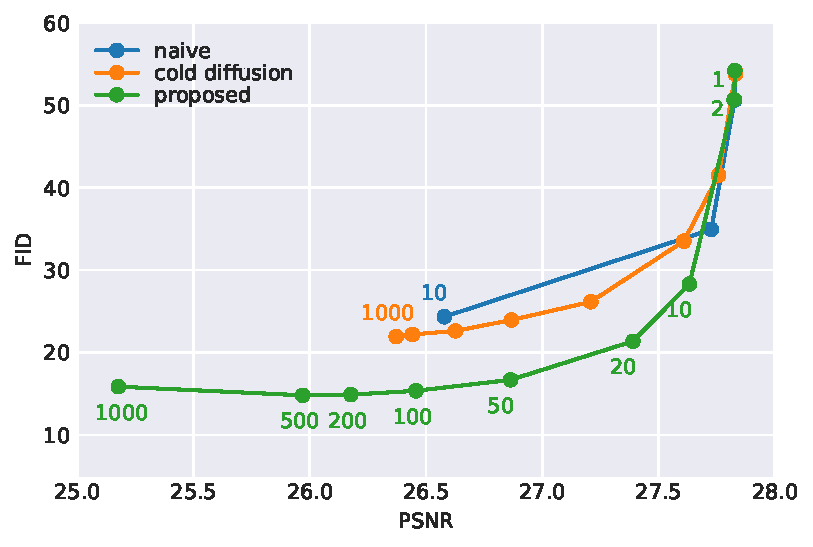
\includegraphics[width=0.95\linewidth]{assets/pd_curve_sisr_4x_div2k_sampler.pdf} \vspace{-.5em}
    
        (b) Upscaling $4\times$ (div2k dataset)
    \end{minipage}
    
    \vspace{.5em}
    \begin{minipage}[c]{.48\textwidth}
    \centering
    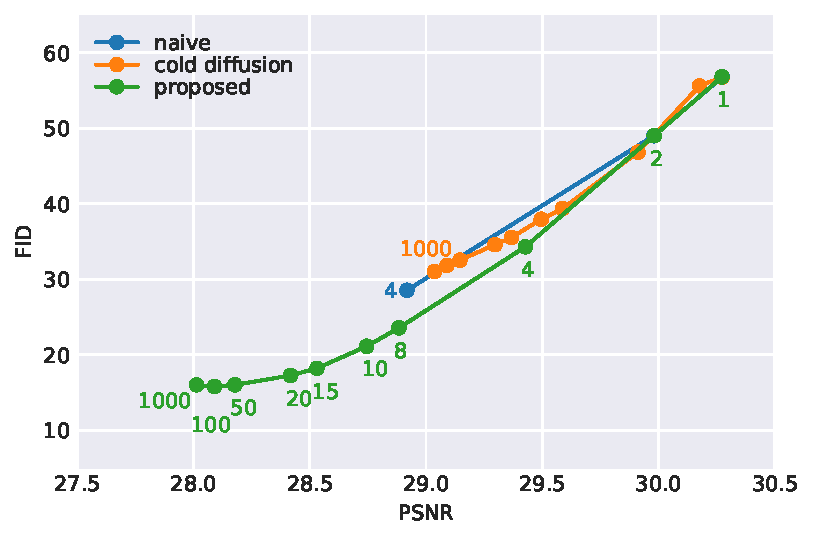
\includegraphics[width=0.95\linewidth]{assets/pd_curve_dejpeg_q15_sampler.pdf}

        (c) De-Jpeg Q15 (div2k dataset) \vspace{-.5em}

    \end{minipage}
    \begin{minipage}[c]{.48\textwidth}
    \centering
    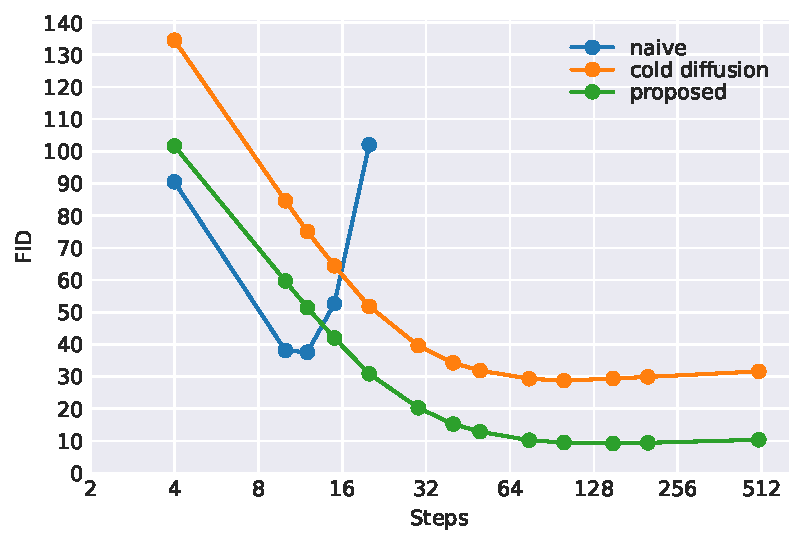
\includegraphics[width=0.95\linewidth]{assets/fid_celebA_gen_sampler.pdf}

     (d) Generative imaging CelebA $64\times64$

    \end{minipage}
    
    
    

    

    
    \caption{Impact of the Inference Algorithm for some of the different tested tasks. The naive inference algorithm (\eqref{eq:naive_sampler}) produces a good baseline when used with very few steps (i.e. 2--5) but then diverges. The proposed updated rule (\eqref{eq:baseline_sampler}) produces better results than the one adapted from Cold Diffusion~\citep{bansal2022cold} given in (\eqref{eq:cold_diffusion_sampler}). At very large number of steps, Cold Diffusion seems to be the most stable of the three tested samplers.  Each of the points in each shown curve represents the results with a different number of steps (similar to what is shown in Figure
   ~\ref{fig:gopro_steps}. Points that leads to values that are out-of-the shown region are left out for improving visualization. }
    \label{fig:impact_sampler}
\end{figure}